\documentclass[20pt, a0paper, landscape,colspace=1cm]{tikzposter}

% \usepackage[utf8]{inputenc}
 
\title{OPTIMAL FISHING RATES FOR MULTIPLE FLEETS}
\author{Steven Martell and Catarina Wor}
\date{\today}
\institute{INTERNATIONAL PACIFIC HALIBUT COMMISSION}
 
\usepackage{blindtext}
\usepackage{comment}

% Themes
\usetheme{Default} 
%\usetheme{Rays} 
% \usetheme{Basic} 
% \usetheme{Simple} 
% \usetheme{Envelope} 
% \usetheme{Wave} 
% \usetheme{Board} 
% \usetheme{Autumn} 
% \usetheme{Desert} 


% Block styles
\useblockstyle{Default}
\useblockstyle{Basic}
\useblockstyle{Minimal}
\useblockstyle{Envelope}
\useblockstyle{Corner}
\useblockstyle{Slide} 
\useblockstyle{TornOut}

% Note styles
\usenotestyle{Sticky}


% Note colors
\definecolor{notefgcolor}{named}{black}
\definecolor{notebgcolor}{HTML}{FCF0AD}



% additional packages
% \usepackage{times}
\usepackage{amsmath,amsthm, amssymb, latexsym, bm}
% \usepackage{exscale}
% \usepackage{ragged2e}
% \boldmath
% \usepackage{booktabs, array}
% \usepackage{rotating} %sideways environment
\usepackage[english]{babel}
\usepackage[latin1]{inputenc}
% \listfiles
% \graphicspath{{figures/}}
% \graphicspath{{FIGS/}}




% abbreviations
\usepackage{xspace}
\makeatletter
\DeclareRobustCommand\onedot{\futurelet\@let@token\@onedot}
\def\@onedot{\ifx\@let@token.\else.\null\fi\xspace}
\def\eg{{e.g}\onedot} \def\Eg{{E.g}\onedot}
\def\ie{{i.e}\onedot} \def\Ie{{I.e}\onedot}
\def\cf{{c.f}\onedot} \def\Cf{{C.f}\onedot}
\def\etc{{etc}\onedot}
\def\vs{{vs}\onedot}
\def\wrt{w.r.t\onedot}
\def\dof{d.o.f\onedot}
\def\etal{{et al}\onedot}
\makeatother




\newcommand{\fspr}{F$_{\rm{SPR=35\%}}$}
\newcommand{\bspr}{B$_{\rm{SPR=35\%}}$}
\newcommand{\rspr}{R$_{\rm{SPR=35\%}}$}
\newcommand{\fofl}{F$_{\rm{OFL}}$}

\usepackage{pifont}% http://ctan.org/pkg/pifont
\newcommand{\cmark}{\ding{51}}%
\newcommand{\xmark}{\ding{55}}%

% \newcommand{\fmsy} {F$_{\rm{\textbf{MSY}}}$}
\newcommand{\fmsy}   {$f^*$}

\newcommand{\dye}    { \dfrac{{\partial y_k}}{{\partial f_k}} }%
\newcommand{\dre}    { \dfrac{{\partial R_e}}{{\partial f_k}} }%
\newcommand{\drep}    { \dfrac{{\partial R_e}}{{\partial f_{k'}}} }%
\newcommand{\dphi}   { \dfrac{{\partial \phi_k}}{{\partial f_k}} }%
\newcommand{\dphip}  { \dfrac{{\partial \phi_{k}}}{{\partial f_{k'}}} }%
\newcommand{\dqak}   { \dfrac{{\partial q_{k,a}}}{{\partial f_k}} }
\newcommand{\dqakp}   { \dfrac{{\partial q_{k,a}}}{{\partial f_{k'}}} }
\newcommand{\dphie}  { \dfrac{{\partial \phi_e}}{{\partial f_k}} }%
\newcommand{\ddphie} { \dfrac{{\partial^2 \phi_e}}{{\partial f_k}^2} }%
\newcommand{\dla}    { \dfrac{{\partial l_a}} {{\partial f_k}}}%
\newcommand{\dlap}    { \dfrac{{\partial l_a}} {{\partial f_{k'}}}}%
\newcommand{\ddla}   { \dfrac{{\partial^2 l_a}} {{\partial f_k}^2} }%
\newcommand{\ddlap}   { \dfrac{{\partial^2 l_a}} {{\partial f_{k'}}^2} }%
\newcommand{\ddye}   { \dfrac{{\partial^2 y_k}}{{\partial f_k'}^2} }%
\newcommand{\ddre}   { \dfrac{{\partial^2 R_e}}{{\partial f_k}^2} }%
\newcommand{\ddrep}   { \dfrac{{\partial^2 R_e}}{{\partial f_{k'}}^2} }%
\newcommand{\ddphi}  { \dfrac{{\partial^2 \phi_k}}{{\partial f_k}^2} }%
\newcommand{\ddphip}  { \dfrac{{\partial^2 \phi_k}}{{\partial f_{k'}}^2} }%
\newcommand{\ddqak}   { \dfrac{{\partial^2 q_{k,a}}}{{\partial f_k}^2} }
\newcommand{\ddqakp}   { \dfrac{{\partial^2 q_{k,a}}}{{\partial f_{k'}}^2} }
\newcommand{\ddphik} { \dfrac{{\partial^2 \phi_{k'}}}{{\partial f_k}^2} }%



\definecolor{cM1}{rgb}{0.9608,0.4706,0.4392}
\definecolor{cM2}{rgb}{0.4902,0.6745,0.1216}
\definecolor{cM3}{rgb}{0.2275,0.7765,0.7922}
\definecolor{cM4}{rgb}{0.7765,0.5020,0.9843}


\begin{document}
 
\maketitle

\begin{columns}
	\column{0.25}
	\block{Problem}
	{
	When there are two or more distinctly different gear types (i.e., hook \& line versus trawl) harvesting the same stock, determining the optimal fishing mortality rates for each gear is largely determined by selectivity.\\

	There are two distinctly different optimization problems: (1) to maximize the total yield across all fisheries, and (2) to maximize the total yield under a allocation agreement or catch shares (Fig. \ref{fig.MSY}).
	}
	%%
	%%
	\column{0.25}
	\block{Objective}
	{
		The objective of this poster is to show how to derive estimates of optimal fishing mortality rates can be simultaneously derived for each fishery.  
	}
	%%
\end{columns}

% \begin{columns}
%     \column{0.4}
%     \block{More text}{Text and more text \blindtext}
 
%     \column{0.6}
%     % \useblockstyle{Slide} 
%     \block{Something else}{Here, \blindtext \vspace{4cm}}
%     \note[
%         targetoffsetx=-9cm, 
%         targetoffsety=-16.5cm, 
%         width=0.35\linewidth
%         ]
%         {e-mail \texttt{stevem@iphc.int}\\
        
%         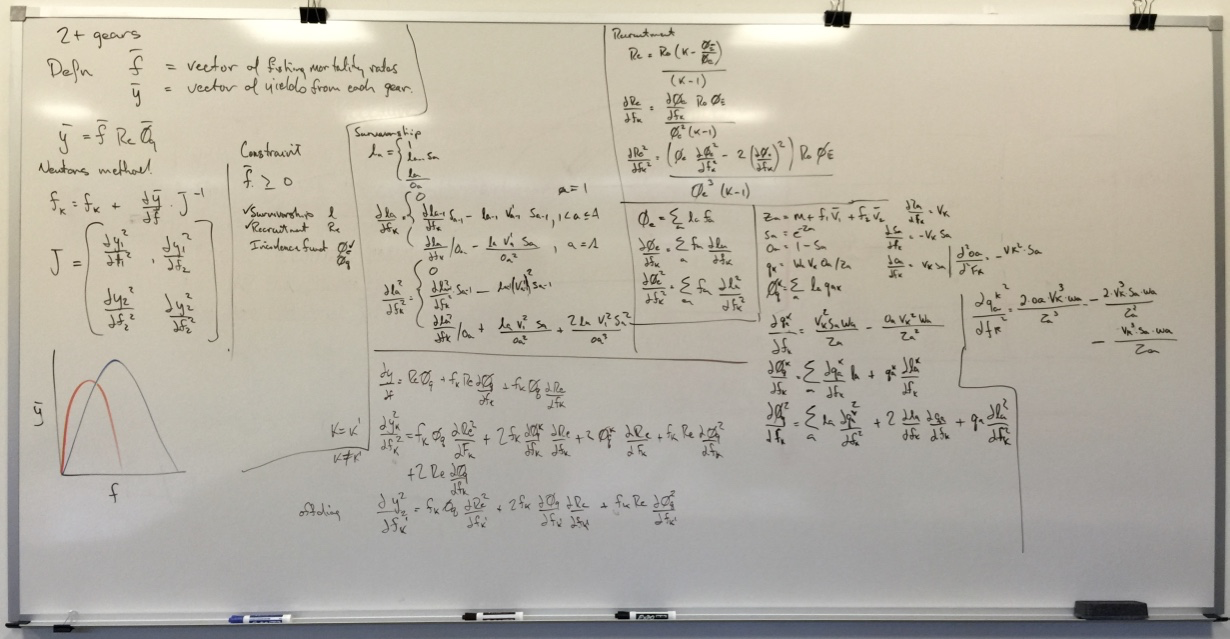
\includegraphics[width=0.95\linewidth,keepaspectratio=true]{./whiteBoard.png}}

% \end{columns}

\begin{columns}
	% 
	% CATCH EQUATIONS
	% 
	\column{0.28}
	\block{Catch Equation \& Finding $\bm{f^*}$}{
		Assuming all fisheries and natural mortality operate simultaneously, the equilibrium catch equation for each fleet can be written as a vector
		\begin{align}
			%
			\vec{y} = \vec{f} R_e \vec{\phi}  \label{eq.1}
			%
		\end{align}
		To find the vector of fishing mortality rates that simultaneously maximizes the yield for each fleet we use Newton's method to find the solution to $\dfrac{\partial \vec{y}}{\partial \vec{f}} = 0$.  The first and second derivatives of \eqref{eq.1} for fleet $k$ are given by:
		\begin{align}
			%
			\mbox \nonumber \\
			\dye &=
			\begin{cases}
			 R_e \phi_k + f_k R_e \dphi +  f_k \phi_k \dre & k = k' \\[1ex]
			%
			 f_k R_e \dphip + f_k \phi_k \drep  & k \neq k' 
			\end{cases} \label{eq.2}
			%
			\\ \nonumber
			\\ \nonumber
			\mbox{Jacobian} \nonumber \\
			\ddye &=
			\begin{cases}
				f_k \phi_k \ddre + 2 f_k \dphi \dre + 2 \phi_k \dre + f_k R_e \ddphi + 2 R_e \dphi & k = k' \\[3ex]
				%
				f_{k} \phi_k \ddrep + 2 f_{k} \dphip \drep + f_{k} R_e \ddphip & k \neq k'
			\end{cases} \label{eq.3}
		\end{align}
		The difficulty is in calculating all of the partial derivatives.  We break this down into suvivorship, recruitment, and per-recruit functions. The Newtons iteration step is given by:
		\begin{align}
			\vec{f}_{i+1} = \vec{f}_{i} - \dfrac{\partial y}{\partial f}
			 \left( \dfrac{{\partial y}^2}{{\partial f}^2} \right)^{-1} \label{eq.4}
		\end{align}
	}% end block.

	% 
	% MATH SYMBOLS USED IN EQUATIONS
	% 
	\note[
		width=11cm,
		targetoffsetx=-10.5cm,
		targetoffsety=-12cm,
		rotate=00,
		angle=0,
		radius=0cm,
		connection
		]
	{	
		\textbf{Symbols}\\
		\begin{tabular}{cl}
			$\vec{f}$     & fishing mortality rates.\\
			$\vec{y}$     & equilibrium yields.\\
			$\vec{\phi}$  & yield per recruit.\\
			$R_e $        & equiliibrium recruitment.\\
		\end{tabular}
	}

	% 
	% SURVIVORSHIP
	% 
	\column{0.28}

	\block{Survivorship}{
		The age-specific total mortality rate and survival rate is defined as \[ z_a = M_a + \sum_k f_k v_{k,a}, \quad s_a = \exp(-z_a).\]
		The survivorship of a cohort is based on the following recurstive function:
		\begin{align}
			l_a &= \begin{cases}
				1,  & a = 1\\[1ex]
				l_{a-1} s_{a-1}, & 1<a<A\\[1ex]
				\dfrac{l_{a}}{1 - s_{a}}, & a = A
			\end{cases}\label{eq.5} \\[1ex]
		\end{align}
		and the vectors of first and second derivatives are:
		\begin{align}
			\dla &= \begin{cases}
				0, & a=1\\[1ex]
				% 
				s_{a-1} \cdot\left(\dfrac{\partial l_{a-1}}{\partial f_k} - l_{a-1}v_{k,a-1} \right),   &1 < a < A \\[3ex]
				% 
				\dfrac{1}{\left(1-s_a \right)} \cdot
				\left[
				{{s}_{a-1}} \cdot \left(\dfrac{\partial l_{a-1}}{\partial f_k}-{{l}_{a-1}} {{v}_{a-1}} \right) 
				 - \dfrac{{{l}_{a-1}} {{s}_{a-1}}  {{v}_{k,a}} { s_{a}} }
					{{{\left( 1-{s_{a}}\right) }}}
					\right], & a = A 
			\end{cases}\label{eq.7} \\[3ex]
			% 
			% 
			\ddla & = \begin{cases}
				0, & a = 1\\[1ex]
				%
				 { s_{a-1} }\cdot \left(
				\dfrac{{\partial^2 l_{a-1}}} {{\partial f_k}^2}
				+ {{l}_{a-1}} {{v}_{k,a-1}^{2}} 
				+ 2  \dfrac{{\partial l_{a-1}}} {{\partial f_k}} v_{k,a-1}
				\right), & 1<a<A\\[3ex]
				%
				 \dfrac{1}{\left(1-s_a \right)} \cdot
				{ s_{a-1} }\cdot \left(\dfrac{{\partial^2 l_{a-1}}} {{\partial f_k}^2} + {{l}_{a-1}} {{v}_{k,a-1}^{2}} 
				+ 2  \dfrac{{\partial l_{a-1}}} {{\partial f_k}} v_{k,a-1}
				\right) \\
				 + \dfrac{ {{l}_{a-1}} {{s}_{a-1}}  {{v}_{k,a}^{2}} {{s}_{a}} } { (1- s_a)^2 } 
				 +\dfrac{ 2  {{l}_{a-1}}  {{s}_{a-1}}  {{v}_{k,a}^{2}}  {{s}_{a}}^2 } 
				      {(1-s_a)^3} \\
				- \dfrac{2 \cdot s_{a-1} \cdot\left(\dfrac{\partial l_{a-1}}{\partial f_k} - l_{a-1}v_{k,a-1} \right) \cdot
				 {v}_{k,a} {s}_{a}} {(1-s_a)^2}  
				 & a = A 				 
			\end{cases} \label{eq.8}
		\end{align}
	}

	% 
	% MATH SYMBOLS USED IN SURVIVORSHIP
	% 
	\note[
		width=11cm,
		targetoffsetx=-10.5cm,
		targetoffsety=12cm,
		rotate=00,
		angle=0,
		radius=0cm,
		connection
		]
	{	
		\textbf{Symbols}\\
		\begin{tabular}{cl}
			$M_a$     		& natural mortality.\\
			$v_{k,a}$  	 	& selectivity for gear $k$.\\
			$f_k$			& fishing rate for gear $k$.\\
			$s_a$  			& survival rate at age $a$.\\
			$l_a $      	& survivorship to age $a$.\\
		\end{tabular}
	}


	% 
	% RECRUITMENT
	% 
	\column{0.2}
	\block{Recruitment}{
		The following assumes that recruitment follows a Beverton-Holt relationship parametrized using the inverse of the spawning potential ratio:
		\begin{align}
			R_e &= R_o \frac{(\kappa-\phi_{E}/\phi_{e})}{(\kappa - 1)}\label{eq.9}
		\end{align}
		The first and second derivatives, required in \eqref{eq.3} and \eqref{eq.4}, are given by:
		\begin{align}
			\dre &= \dphie \cdot \frac{R_o \phi_{E}}{(\kappa -1) \phi_{e}^2} \label{eq.10} \\[3ex]
			%
			%
			\ddre &= \dfrac{R_o \phi_{E}
			\left[\phi_{e} \cdot \ddphie 
			- 2 \cdot \left(\dphie\right)^2 \right]}
			{\phi_e^3 (\kappa -1)}\label{eq.11}
		\end{align}
	}

	% 
	% MATH SYMBOLS USED IN RECRUITMENT
	% 
	\note[
		width=15cm,
		targetoffsetx=-5cm,
		targetoffsety=-11cm,
		rotate=-2
		]
	{	
		\textbf{Symbols}\\
		\begin{tabular}{cl}
			$R_e$     		& equilibrium recruitment.\\
			$R_o$  	 		& unfished recruitment.\\
			$\kappa$		& recruitment compensation ratio.\\
			$\phi_{e} $     & spawning biomass per recruit.\\
			$\phi_{E} $     & unfished spawning biomass per recruit.\\
		\end{tabular}
	}

	% 
	% PER RECRUIT FUNCTIONS
	% 
	\column{0.24}
	\block{Per Recruit Functions}{
		The spawning biomass per recruit is the sum of products of survivorship and mature biomass at age:
		\begin{align}
			\phi_{e} &= \sum_a l_a w_a m_a \label{eq.12}
		\end{align}
		and $\phi_{E}$ is the same as \eqref{eq.12} where survivorship is based only on natural mortality (i.e., $f_k=0, \quad \forall k$).\\
		The first and second derivatives of $\phi_{e}$ are given by

		\begin{align}
			\dphie &= \sum_a f_a \cdot \dla  \label{eq.13}
		\end{align}

		\begin{align}
			\ddphie &= \sum_a f_a \cdot \ddla  \label{eq.14}
		\end{align}

		Yield per recruit $\phi_k$ for fishery $k$ is based on the Barnov catch equation:
		\begin{align}
			q_{k,a} &= w_a v_k (1-s_a)/ z_a \nonumber \\
			\phi_k &= \sum_a l_a q_{k,a} \label{eq.15}
		\end{align}
		The derivative of the yield per recruit with respect to $f_k$ is given by
		\begin{align}
		\dphip &=
			\begin{cases}
				 \dqak \cdot l_a + \dla \cdot q_{a,k} & k = k'\\
					%
				 \dqakp \cdot l_a + \dlap \cdot q_{a,k} & k \neq k'
			\end{cases}
		\end{align}
		Where:
		\begin{align}
		\dqakp &=
			\begin{cases}
				 \dfrac{{v_k}^{2} \cdot w_a}{z_a} \cdot \left( s_a- \dfrac{1-s_a}{z_a}\right) & k = k' \\
				%
				\dfrac{{v_k}\cdot v_{k'} \cdot w_a}{z_a} \cdot \left( s_a- \dfrac{1-s_a}{z_a}\right) & k \neq k'
			\end{cases}
		\end{align}
		And second derivative

		\begin{align}
		\ddphip &=
			\begin{cases}
				 \ddqak \cdot l_a + 2 \cdot \dla \dqak + \ddla \cdot q_{a,k} & k = k'\\
					%
				 \ddqakp \cdot l_a + 2 \cdot \dlap \dqakp + \ddlap \cdot q_{a,k} & k \neq k'
			\end{cases}
		\end{align}
		Where:
		\begin{align}
		\ddqakp &=
			\begin{cases}
				 \dfrac{{v_k}^{3} \cdot w_a}{z_a} \cdot \left( - s_a - 2 \cdot \dfrac{s_a}{z_a}+ 2 \cdot \dfrac{1-s_a}{{z_a}^2}\right) & k = k' \\
				%
				\dfrac{{v_k}\cdot v_{k'^2} \cdot w_a}{z_a} \cdot \left( - s_a - 2 \cdot \dfrac{s_a}{z_a}+ 2 \cdot \dfrac{1-s_a}{{z_a}^2}\right) &  k \neq k'
			\end{cases}
		\end{align}
		
	}
	
\end{columns}

\begin{columns}
	\column{1}
	\useblockstyle{Minimal}
	\block{Post-its}{
		\centering
		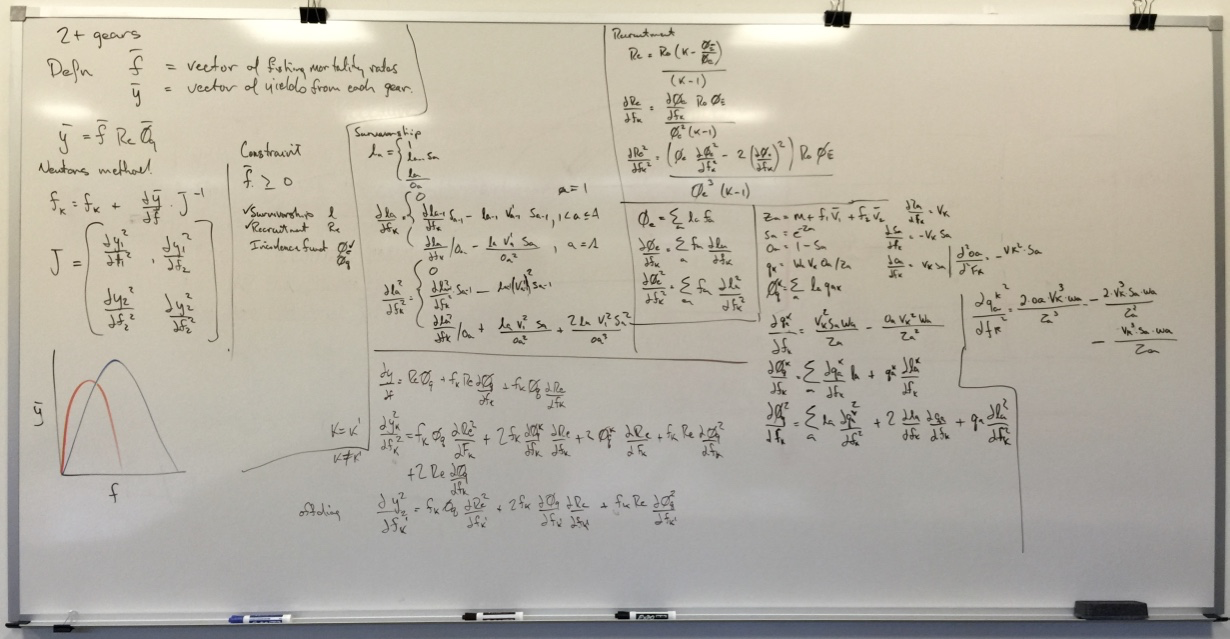
\includegraphics[width=0.30\linewidth,keepaspectratio=true]{./whiteBoard.png}
	}
	\useblockstyle{TornOut}
	%
	% MSY Figure
	% 
	%\note[
	%	width=14cm,height=14cm,
	%	targetoffsetx=-60cm,
	%	targetoffsety=+3cm,
	%	rotate=05
	%	]{
	%	%Figure environment does not work
	%	\begin{tikzfigure}[Equilibrium yield versus fishing mortality for 2 fishing gears. Which fishery (A or B) catches smaller fish?]
	% 	\label{fig.MSY}
	% 	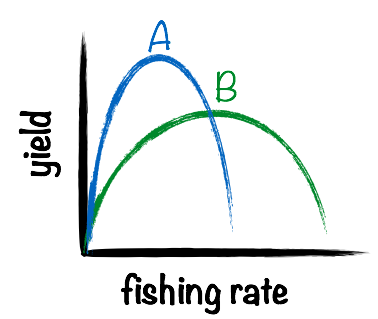
\includegraphics[width=11cm]{figMSY.png}
	%	\end{tikzfigure}
	%}

\end{columns}
		
	

\end{document}